\documentclass[a4paper, 9pt]{article}
\title{FONDAMENTI DI AUTOMATICA}
  
\author{Federico Mainetti Gambera}
\usepackage{amsmath}
\usepackage{amssymb}
\usepackage{graphicx}
\usepackage[italian]{babel}
\usepackage{import}
\usepackage{xifthen}
\usepackage{pdfpages}
\usepackage{transparent}
\usepackage{xcolor}
\usepackage{cancel}
\usepackage[a4paper,left=35mm,top=26mm,right=26mm,bottom=15mm]{geometry}
\usepackage{color}
\usepackage{tcolorbox}
\usepackage{hyperref}
\usepackage{makeidx}
\makeindex
\definecolor{lightgray}{gray}{0.75}
\renewcommand{\familydefault}{\sfdefault}
\newenvironment{rcases}
  {\left.\begin{aligned}}
  {\end{aligned}\right\rbrace}
\newcommand{\incfig}[1]{%
    \def\svgwidth{\columnwidth}
    \import{../images/}{#1.pdf_tex}
}
\begin{document}
    \maketitle
    \tableofcontents{}
    %lezioni
    \newpage
    \part{Lezioni}
%\begin{comment}
    \section{LEZIONE 1 11/03/20}
https://web.microsoftstream.com/video/58568b1d-5fc5-41c0-88f6-608e4b8f9f7a
\subsection{Calendario delle lezioni}
https://docs.google.com/spreadsheets/d/14ShTdkFCZ63MlyKP0LCSLPsPAeiu8D2sYVXSrkw9B6k/edit#gid=0
\subsection{Introduzione al corso}
Non ci saranno prove in itinere per questo corso.\newline
E' opportuno guardare i video relativi agli argomenti indicati prima di partecipare alla lezione.\newline
Queste lezioni hanno lo scopo di aggiungere informazioni, chiarire dubbi e aiutarci a capire quali siano gli argomenti più importanti e i punti chiave.\newline
I materiali video coprono interamente gli argomenti del corso.\newline
\subsection{HTTP}
Il web è una piattaforma per sviluppo di applicazioni con un architettura molto particolare. Per architettura si intende l'insieme delle risorse (hardware, connettività, software di base, software applicativo).\newline
Le applicazioni web hanno una particolare conformazione della loro architettura che prevede tre livelli: Client, Middle-tier, Data-tier.\newline 
Le architetture sono  cambiate molto negli anni. Se ne individuano tre grandi famiglie: Mainframe, Client-Server, Multi-tier (per esempio le applicazioni web). \newline
Il compito di questo corso è quello di riuscire a programmare nel Middle-tier con qualche accenno al Client.\newline
In un'applicazione web il Client interagisce con il Middle-tier con un preciso protocollo, che non è quello tcp-ip. Parliamo del protocollo HTTP.\newline
Una lettura molto importante per il corso è il documento RequestforComment 1945, Tim Berners Lee (https://www.w3.org/Protocols/rfc1945/rfc1945), che rappresenta l'atto di fondazione del web.\newline
Il Client manda delle request al Server che invia delle responses. Le request del Client sono gestite tramite un applicazione detta User agent (browser).\newline
Le richieste del Client e le risposte del server sono delle semplici stringhe. Http è rivoluzionario per la sua semplicità.\newline
Architettura delle applicazioni web: c'è un client (pc) con un user agent (browser) che emette richieste che vengono servite con delle risposte da un web server, detto anche HTTP server. L'archiettura di cui però ci occupiamo è più complicato di così, perchè vede alle spalle del web server un application server (TomCat), che ha lo scopo di calcolare una risposta e consegnarla al web server per rimandarla al client.\newline
Bisogna installare un'archiettura completa sul pc che prevede tutti i livelli appena visti (guida nella cartella strumenti) (si può usare anche IntellyJ invece di Eclipse).\newline
Altri elementi dell'architettura sono il proxy e il gateway. Il proxy è un intermediario fra un client e un origin server, per definizione può comportarsi sia come server sia come client. Fa copie di risorse e le inoltra ai client e può essere anche utile per limitare gli accessi e gestire autorizzazioni. Il Gateway serve per far interagire un applicazione web con applicazioni che non usano il protocollo HTTP, quindi il gateway traduce richieste HTTP per applicazioni che non lo comprendono, tipicamente usato per SQL.\newline
Come si identifica una risorsa? con URL (Uniform Resourse Locator) che è una striga formatta in maniera molto semplice: prefisso (protocollo),indicazione della macchina fisica in cui è presente la risorsa, una eventuale porta in cui la macchina ascolta le richieste, un Path. Gli URL sono estremamenti semplici, e utilizza concetti che esistevano già.\newline
HTTP request: è una banale stringa che contiene una request-line, degli header e un allegato (per gli upload) facoltativi. la request-line è strutturata così: il metodo (funzione) della richiesta, l'URL, la versione del protocollo usata. I metodi di richiesta sono principalmente due, GET e POST; questi metodo possono essere visti come chiamate di funzione.\newline
HTTP response: anche questa è una banale stringa, che, ancora più semplicemente contiene un codice di stato (es. 404 file not found), degli header facoltativi, e un allegato.\newline
La conseguenza di un protocollo così semplice è che con un solo client si può interagire con tutti i back end. La complessità si sposta però nell'application server.\newline
Gli header sono informazioni opzionali a cura del browser, trasmesse come fossero parametri che aggiungono informazioni alla request o alla response.\newline

    \section{LEZIONE 2 12/03/2020}
\textbf{link} \url{https://web.microsoftstream.com/video/7f38ca42-5bcf-4a08-b9cf-d42ca1289062}
\subsection{Cinematica di un corpo}
\subsubsection{Definizioni}
\begin{itemize}
    \item Corpo: Un corpo è un insieme continuo di infiniti punti che assume dimensioni finite.
    \item Posizione del corpo: è l'insieme di tutti i vettori posizione relativi a ciascun punto appartenente al corpo.
    \item Spostamento, velocità, accellerazione: definiziamo spostamento, velocità, accellerazione, l'insieme di tutti i vettori spostamento, velocità, accellerazione relativi a ciascun punto appartenente al corpo.
    \item Moto piano: in questo corso faremo sempre riferimento a un moto piano, che rappresenta il caso in cui tutti i vettori posizione, velocità e accellerazione di tutti i punti appartenenti al corpo sono paralleli a un piano, detto piano direttore.
    \item Spostamento infinitesimo: lo spostamento infinitesimo è una condizione di moto per cui ogni punto che appartiene al corpo subirà uno spostamento di dimensione infinitesima.
    \item Atto di moto: l'atto di moto è l'insieme delle velocità di tutti i punti che appartengono al corpo nell'istante di tempo geneico considerato. L'atto di moto rappresenta una "fotografia istantanea" del suo campo di velocità. Possiamo definire un'analogia fra lo spostamento infinitesimo e l'atto di moto: siccome la velocità di un generico punto $P$ è $\vec{v_P} = \frac{d \vec{P}}{dt}$, l'atto di moto può essere visto come lo spostamento infinitesimo di $P$ fratto l'intervallo di tempo infinitesimo $dt$ in cui esso avviene. Perciò tutte le regole cinematiche che definiremo per l'atto di moto varranno anche per lo spostamento infinitesimo.
\end{itemize}
Tutte le definizione appena viste valgono per un qualsiasi corpo, ma noi nel corso vedremo solo corpi rigidi.\newline
Per un corpo deformabile ci servono $\infty^2$ gradi di libertà (caso piano) per descrivere ciascuno degli infiniti punti che lo rappresentano.\newline
Nel caso di un corpo rigido saranno sufficienti $3$ gradi di libertà per definire la posizione del corpo nel piano.
\subsubsection{Corpo rigido}
Un corpo si definisce rigido se esso può definire solamente spostamenti rigidi. Uno spostamento si può definire rigido se a fronte di esso il corpo non subisce alcuna variazione nè di forma nè di dimensioni.\newline
[immagine dagli appunti del prof]\newline
Più analiticamente diciamo che uno spostamento è rigido se a seguito dello spostamento esiste un nuovo sistema di riferimento per cui la posizione del corpo rigido risulta la stessa di partenza.\newline
Se per esempio il corpo subisce un rimpicciolimento o una deformazione a seguito dello spostamento, non siamo in presenza di uno spostamento rigido.\newline
Ne conseguono due proprietà:
\begin{itemize}
    \item La distanza fra due punti qualsiasi di un corpo rigido si mantiene immutata.
    \item L'angolo formato dalle rette passanti fra due coppie di punti appartenenti al corpo rimane immutato.
\end{itemize}
Il principale vantaggio di studiare corpi rigidi è che dobbiamo usare solo 3 coordinate (3 gradi di libertà) per descrivere pienamente degli spostamenti.\newline
[immagine del professore]\newline
Per capire quali tre coordinate scegliere si seleziona un punto qualsiasi $A$ all'interno del corpo:
\begin{itemize}
    \item la prima è l'ascissa del punto $A$ (come per il punto), $x_A(t)$;
    \item la seconda è l'ordinata del punto $A$ (come per il punto), $y_A(t)$.
    \item La terza è la coordinata angolare $\phi$ di un segmento qualsiasi che collega il punto $A$ con un altro generico punto $B$ interno al corpo. Ogni punto $B$ mantiene invariata la sua distanza dal punto $A$ a seguito di un qualsiasi spostamento e, studiando come varia l'orientamento di questo segmento $AB$, sono in grado di ricostruire la posizione di ciascuno dei punti all'interno del corpo rigido. La rotazione $\phi$ avviene attorno ad un asse $z$ che esce dal piano del corpo rigido. Qualsiasi segmeno all'interno del corpo subirà la stessa variazione angolare (stessa rotazione): la rotazione $\phi$ è una proprietà dell'intero corpo rigido.
\end{itemize}
\subsubsection{Moto in grande}
\begin{itemize}
    \item \textbf{Traslazione}: é un moto nel quale un corpo non varia il proprio orientamento, ovvero in cui la coordinata angolare rimane costante. Tutti i punti del corpo subiranno lo stesso esatto spostamento, dunque $\vec{v_A} = \vec{v_B} = \dots$, $\vec{a_A} = \vec{a_B} = \dots$ e le traiettorie di ciascun punto saranno le stesse.
    \newline[immagine dagli appunti del prof]
    \item \textbf{Rotazione}: è un moto nel quale un punto (anche esterno al corpo), detto centro di rotazione, che mantiene la sua posizione fissa durante lo spostamento. Tutti gli altri punti invece subiranno una rotazione $\phi$. La traiettoria di ogni punto seguirà un moto circolare. Possiamo definire un vettore detto $\vec{\phi} = \phi \vec{k}$ ovvero con direzione uscente dal piano.
    \newline[immagine dagli appunti del prof]
    \item \textbf{Rototraslazione}: il corpo rigido andrà a modificare la propria posizione senza però che sia possibile individuare un punto che rimane fermo. Per studiare il moto rototraslatorio si può lavorare considerando due spostamenti successivi, prima una traslazione e poi una rotazione.
    \newline[immagine dagli appunti del prof]
\end{itemize}
\subsubsection{Atto di moto (moto in piccolo)}
Per atto di moto si intende un moto in cui gl ispostamenti e le rotazioni sono di dimensione infinitesima. L'atto di moto rappresenta una "fotografia istantanea" del campo di velocità del corpo.\newline
Andando ad osservare movimenti in piccolo quindi ci ritroviamo difronte a moti o rotatori o traslatori, non rototraslatori. Se la velocità di tutti i punti è uguale in modulo direzione e verso, l'atto di moto è di tipo traslatorio. Viceversa, se esiste un punto, detto centro di istantanea rotazione, in cui la velocità è nulla, siamo in presenza di un moto di tipo rotatorio.\newline
\textbf{es.} Esempio di rotazione:\newline
[immagine dagli appunti del prof]\newline
Presi i punti $A$ e $B$ interni al corpo e le rispettive velocità $\vec{v_A}$ e $\vec{v_B}$, essendo il corpo rigido, le proiezioni delle velocità sulla retta $r_{AB}$ devono essere di medesima lunghezza (nell'immagine evidenziate in giallo).\newline
Consideriamo ora le rette $r_A$ passante per $A$ e perpendicolare a $\vec{v_A}$ e la retta $r_B$ passante per $B$ e perpendicolare a $\vec{v_B}$; tutti i punti che si trovano sulla retta $r_A$ devono avere velocità perpendicolare alla retta stessa (analogo per la retta $r_B$), perchè altrimenti il corpo subirebbe una deformazione, quindi tutti i punti su $r_A$ (o $r_B$) devono avere velocità perpendicolare a $\vec{v_A}$ (o $\vec{v_B}$). Il punto $C$ di intersezione di queste due rette dovrebbe avere velocità perpendicolare sia a $\vec{v_A}$ sia a $\vec{v_B}$, ma questo è possibile solo se $\vec{v_C} = 0$, dunque il punto $C$ è il centro di istantanea rotazione del corpo rigido e siamo dunque in presenza di una rotazione.\newline
Il centro di istantanea rotazione differisce dal centro di rotazione (dei moti in grande), il primo ha velocità nulla solo nell'istante che stiamo considerando, mentre il secondo è fermo per tutto l'arco della rotazione. In poche parole il centro di istantanea rotazione ha velocità nulla, ma la sua accellarazione può non esserlo.\newline
\textbf{es.} Esempio di traslazione:\newline
[immagine dagli appunti del prof]\newline
In questo caso le rette $r_A$ e $r_B$ sono parallele e non si incontrano mai, il centro di istantanea rotazione non è definibile e dunque il moto e traslatorio.\newline
\textbf{es.} Esempio di moto di un corpo non rigido:\newline
[immagine dagli appunti del prof]\newline
Se i due punti $A$ e $B$ hanno $\vec{v_A}$ e $\vec{v_B}$ di modulo diverso, le proiezioni di queste due velocità sulla retta $r_{AB}$ non sono identiche e dunque il corpo si sta deformando.\newline
\textbf{es.} Un altro esempio di rotazione:\newline
[immagine dagli appunti del prof]\newline
Se i due punti $A$ e $B$ hanno $\vec{v_A}$ e $\vec{v_B}$ di direzione opposta, la congiungete fra le due velocità (disegnata in rosso) ci mostra che la velocità di tutti i punti lungo il segmeno $AB$ deve diminuire man mano che ci avviciniamo al punto $C$, che quindi ha velocità nulla e rappresenta il centro di istantanea rotazione.
    \title{LEZIONE 3 18/03/20}\newline
\textbf{link} \href{https://web.microsoftstream.com/video/53d9a40e-3109-44fc-8195-0553eedfb6d9}{clicca qui}
\subsection{Esempi}
Una programmazione in servlet è una programmazione che ci chiede di rispettare alcune regole per trarne dei benefici. I benefici principali sono la scalabilità, la gestione automatica dei cicli di vita, il mascheramento degli aspetti tecnici di HTTP. Java servlet ci permette di interagire com HTTP attraverso degli oggetti. Uno dei primo esempio di oggetto che si incontra è l'oggetto request.
\subsubsection{Esempio: contatore condiviso fra i client}
Il file web.xml ci permette di controllare le impostazioni con cui vogliamo lavorare, inoltre ci permette di definire parametri a livello di applicazione (globali) o parametri a livello di servlet.\newline
I parametri possono poi essere reperiti con chiamate di metodi di oggetti di sistema in maniera molto semplice.\newline
Con questo esempio, oltre a mostrare l'utilizzo di questi parametri, viene mostrata l'utilità dei dati membro all'interno della servlet (gli attributi dell'oggetto servlet). Esistendo una sola istanza di servlet per tutte le request, ci aspettiamo che i dati membro vengano usati in maniera concorrente per tutti i client.\newline
Nell'esempio particolare del contatore possiamo vedere che tutti i client possono incrementare il valore del contatore, perchè condividono il dato membro della servlet.\newline
Quindi con questo esempio si imparano due cose importanti: come si configura una servlet per farla partire e il particolare modello di gestione della concorrenza e delle variabili.
\subsubsection{Esempio: contatore per ogni client}
Con questo esempio andiamo ad analizzare il meccanismo di una sessione. Per sessione si intende un gruppo di richieste che possono essere fatte risalire a un unico cliente. HTTP ha solo il metodo GET e POST, e quindi sembra che non sia lui ad occuparsi della gestione della sessione, infatti la gestione della sessione non era nativamente intesa all'interno del protocollo HTTP, ma si è sviluppata successivamente grazie all'utilizzo degli header, in particolare esistono due tecnica: o l'uso degli header cookie, oppure grazie all'url rewriting.\newline
Queste due tecniche sono trasparenti per noi programmatori, noi otterremo un oggetto che maschererà i meccanismi che stanno dietro alla gestione delle sessioni.
\subsection{Forme di identificazione}
Il protocollo HTTP nella sua versione più base (senza i metadati aggiuntivi) serve richieste anonime.\newline
\newline
Analiziamo la terminologia e i concetti base che stanno dietro alla sicurezza della gestione delle sessioni (con forme di identificazione del client via via più stringenti):
\begin{itemize}
    \item \textbf{Pseudo identificazione}: l'atto con cui il server associa un'etichetta arbitraria alle richeiste del client allo scopo di identificare quelle che provengono dallo stesso client.\newline
    Come esempio per vedere in atto la pseudo identificazione si può usare il "SessionCounter", aprire due browser (uno in incognito e uno no) e vedere come i due contatori non sono condivisi. La pseudo identificazione non ha bisogno che l'utente effettui il login.
    \item \textbf{Identificazione}: è il processo con cui il cliente dichiara un'identità. Non ci stiamo più riferendo a un client, ma a un user, un account, una persona.
    \item \textbf{Autenticazione}: è il processo in cui il server verifica l'identificazione del client. Il client e il server condividono un "segreto" (password). La differenza fra pseudo identificazione e identificazione-autenticazione è che nel primo il server inventa un label da dare a un client, che comunque rimane anonimo in quanto l'identità è fornita dal server, e nel sencondo il client si dichiara come user e poi viene verificato dal server, quindi in questo caso l'identità proviene dal client.
    \item \textbf{Autorizzazione}: è il processo in cui il server garantisce l'accesso a risorse e processi a un utente identificato e autenticato. L'autorizzazione è una proprietà dell'identità verificata. E' in poche parole il permesso di vedere o fare cose particolari a fronte di un'identità verificata.
    \item \textbf{RBAC} (Role based access control): è uno schema di autorizzazione che garantisce diritti non solo sulla base dell'identità, ma anche sulla base del ruolo.
\end{itemize}
\subsection{Tracciemento della sessione}
Si dice \textbf{cookie} un piccolo contenuto di informazioni che il server installa sul browser del client, allo scopo che venga restituito al server a ogni successiva richiesta per poter tracciare un client e la sua sessione.\newline
\newline
Vediamo ora in maniera "tecnica" come funziona la pseudo-identificazione tramite gli header cookie. Il server, quando riceve la prima richiesta da parte di un client (quindi una richiesta anonima), vuole che la seconda richiesta sia pseudo-identificata (non più anonima), e chiede al client di impostare un label specifico tramite i cookie. Nel momento in cui avviene una richiesta successiva ci accorgiamo che fra i request header è presente, nella voce cookie, il label che il server ha generato e assegnato al client durante la prima interazione.\newline
\newline
Il server propone al client un label tramite l'header set-cookie. Dunque alla seconda richiesta il client restituisce al server questo cookie e quindi riesce a pseudo-identificarsi.\newline
\newline
I cookie non sono un canale sicuro, possono essere sniffati e si possono fare attacchi man-in-the-middle.\newline
\newline
L'identificazione autorizzata non sostituisce la pseudoidentificazione. Immaginiamo che avvenga sia una psaeudo-identificazione, sia una identificazione-autenticazione tramite un login: il Client è stato autenticato e la sessione è tracciata dai cookie. Da ora in poi è ovvio che la sola pseudoidentificazione non implica l'autenticazione precedentemente fatta (altrimenti dei semplici attacchi informatici potrebbero causare grandi problemi di falsa appropriazione di identità), ovvero il tracciamento della sessione e l'identificazione autenticazione sono su due piani diversi.\newline
\newline
Il session tracking implica la psaudoidentificazione del client, o con cookie, dove il server inietta una stringa e il browser la restituisce a ogni futura richiesta, o con url rewriting, ormai non più usato.\newline
\newline
Invece, allo scopo di associare allo pseudo-cliente una qualunque informazione durevole (per esempio l'autenticazione di un client, oppure l'inserimento di un prodotto in un carrello), il server abbina a ogni pseudoidentità un oggetto Java chiamato Session che è controllabile dal programmatore della servlet. In questo oggetto può essere presente un informazione che conferma che questa pseudoidentità è autenticata e corrisponde a un determinato user. L'oggetto Session è nel server container e totalmente all'oscuro del browser, all'intenro si possono depositare informazioni legate a una pseudoidentità (come per esempio il fatto che il client si sia identificato e autenticato).\newline
\newline
Tipiche domande: c'è bisogno del login per personalizzare una pagina? no, basta il concetto di session tracking. A cosa serve il login? Il login serve ad associare ad una pseudoidentità un'identità autenticata allo scopo di fare autorizzazioni.
\subsection{Filtri}
La verifica evento epr evento dei diritti di accesso è una funzionalità obligatoria dei siti multiruolo.\newline
\newline
La verifica viene fatta in ogni controllore e per evitare di duplicare codice si utilizzano i filtri.\newline
\newline
Un filtro è una classe Java che il servler container interpone fra la richiesta (l'HTTP request) e il servizio (la servlet). I filtri possono essere anche concatenati uno dopo l'altro.\newline
\newline
La classe filtro ha sostanzialmente la stessa struttura di una servlet, ha init(), destroy() e invece di doGet e doPost, ha doFilter(). Ci sono tre interfaccie che vengono usate per i filtri e sono: Filter, FilterChain e FIlterConfig.\newline
\newline
La catena di filtri si può specificare nel web.xml, inoltre la catena di filtri è unica per ogni app, non si possono specificare catene particolari per ogni servlet. Il comando chain.doFilter() in poche parole passa il comando al prossimo filtro della catena, se ce ne è uno, altrimenti prosegue passando la richiesta alla servlet che se ne deve occupare.\newline
\newline
    \title{LEZIONE 4 19/03/20}\newline
\textbf{link} \href{https://web.microsoftstream.com/video/53d9a40e-3109-44fc-8195-0553eedfb6d9}{clicca qui}
\section*{Prerequisiti}
Connessione a database con JDBC
\section*{Informazioni}
Informazioni sul progetto.\newline
Nuovo progetto caricato su beep: "Esercizio gestione spese di trasferta", è commentato (slide e readme.md) e contiene una base di dati. Contiene concetti molto improtanti su JDBC.
\section{JDBC}
Gli argomenti di questa lezione verranno corredati alla visualizzazione di un progetto nella cartella su Beep delle lezioni $>$ Servlet-base $>$ Progetto eclipse servlet con jDBC.\newline
\newline
JDBC è un architettura molto elegante per il mondo Java e serve per mettere in contatto applicazioni Java con DB.\newline
JDBC eredita la sua logica da ODBC, un architettura sviluppata originariamente da Microsoft.\newline
\newline
Il vantaggi di JDBC sono legati al mascheramento delle differenze che sono presenti nelle modalità con cui un'applicazione interagisce con una base di dati. Il principale aspetto di JDBC è quello di migliorare la portabilità dei sistemi che fanno uso di DB. Per ottenere questo sfrutta due tecniche: rimuove la necessità che il programmatore conosca le tecnicalità con cui avviene la connessione coi DB, maschera alcune differenze "dialettali" nell'uso di primitive SQL che alcune basi di dati offrono e altre magari offrono in maniera diversa.\newline
\newline
L'architettura JDBC struttura la connessione con la base di dati in maniera intelligente, che consente all'applicazione di ignorare l ospecifico modello della base di dati. Il modello utilizzato è \textbf{stratificato}: l'\textbf{applicazione Java} vede solo un'\textbf{API} (application programming interface) al di sotto del quale c'è un ambiente di runtime che, a fronte di un particolare modello di base di dati, carica un determinato Driver. Per un sistema operatico, un Driver è un programma speciale che contiene le istruzioni di gestione di una determinata periferica, questo stesso meccanismo è stato replicato per sviluppare JDBC.\newline
Più in dettaglio, l'API utilizza un servizio chiamato \textbf{Driver Menager} che ha lo scopo di caricare un determinato \textbf{Driver} a seconda di con quale base di dati dovrà interagire.\newline
\newline
L'effettiva comodità di JDBC risiede nei vantaggi che il programmatore ne trae, ovvero che dovrà interagire con una serie di oggetti di utilità: Connection, Statement, ResultSet, SQLException (Driver e DriverManager li vedremo una sola volta). L'intera architettura JDBC è fatta da queste classi.\newline
\newline
JDBC è utilizzato anche al di fuori dell'ambiente web.\newline
\newline
Per l'uso di JDBC all'interno di una Servlet si usa il seguente workflow (pattern):
\begin{itemize}
    \item connsessione;
    \item preparazione ed esecuzione di query;
    \item precessamento dei risultati;
    \item disconessione (molto importante, siccome la base di dati è una risorsa comune a tutte le servlet, lasciarla "libera" è essenziale, talvolta la disconnessione precede anche il processamento dei risultati; un metodo più avanzato per distribuire in maniera efficiente le connessioni è il cosiddetto "connection pool", più informazioni sul video di questo argomento).
\end{itemize}
Nel momento il programmatore non ha controllo sul ciclo di vita della propria applicazione (come nel caso dei Servlet) si prevedono dei pattern specifici riguardanti le quattro operazioni appena elencate.\newline
\textbf{Connessione}: avviene nel momento di creazione della Servlet, cioè nella funzione init() della Servlet (nelle slide della lezioni ci sono più informazioni sull'esatto procedimento), i parametri (url, utente, pass, modello DB) necessari alla connessione al DB sono tipicamente inseriti all'interno del file xml di configurazione dell'applicazione web;\newline
\textbf{oss.} tutti i blocchi riguardanti l'interazione con DB saranno contenuti in blocchi critici (try... catch... finally).
\textbf{Disconnessione}
    \title{LEZIONE 5 17/03/2020}\newline
\textbf{link} \href{https://web.microsoftstream.com/video/72b5f396-c34b-4ff6-8d6e-44bf6832dd2e?list=user&userId=faa91214-a6f5-40d7-8875-253fd49b8ce1}{clicca qui}
(continuo della lezione scorsa)
\subsection{}
    \title{LEZIONE 6 26/03/20}\newline
\textbf{link} \href{https://web.microsoftstream.com/video/ee54067c-9686-4347-ba02-4b8a9715c174}{clicca qui}
\section{JSTL}
JSP ha una serie di tag attivi (useBean, setProperty, getProperty) che hanno lo scopo di arricchire il template di funzionalità nascondendone il codice dietro a degli elementi pseudo html. In JSP per programmare un custom tag bisogna costruire una classe (tag handler) che implementa un'interfaccia con una serie di metodi (per esempio doStartTag() e doEndTag()) che operano sul contenuto  del tag. Così la programmazione Java diventa completamente trasparente al template. Questa tecnica prende il nome di Code-behind.\newline
\newline
Un primo svantaggio di questo metodo è che nel momento in cui un grafico va ad aprire un file con questi custom tag, non potrà visualizzarlo correttamente in quanto queste marche non possono essere interpretate da un comune editor di html.\newline
Un altro aspetto svantaggioso di permettere di creare tag custom al programmatore è che molti di questi tag finiscono per eseguire la stessa cosa. Per questo motivo si è passati alla standardizzazione di una libreria di tag "universale": JSTL (JSP Standard Tag Library).\newline
\newline
JSTL è un set di standard tag che possono essere usati in modo da evitare la proliferazione di codice duplicato.\newline
\newline
JSTL contiene due componenti:
\begin{itemize}
    \item un linguaggio di espressione EL;
    \item una libreria di tag.
\end{itemize}
Il linguaggio di espressione è EL (expression language) ed è stato inizialmente concepito come sussidio di JSP, ma ora è stato generalizzato per molti linugaggi di programmazione. Il linguaggio è abbastanza articolato, ma noi lo useremo a livello basico (quello che impariamo guardando esercizi e progetti è più che sufficiente).\newline
EL è un linguaggio per la scrittura di espressioni, che sono costrutti la cui valutazione da luogo a un valore (mentre un istruzione è un costrutto che produce un effetto collaterale ed eventualmente produce un valore).\newline
E' particolarmente importante che un linguaggio di espressione sia conciso e facilmente leggibile. EL permette l'accesso diretto agli attributi di uno scope JSP che ha il ruolo di mappa. EL permette anche la navigazione all'interno di una complessa struttura di un oggetto con la dot-notation.\newline
Il contenitore a cui si fa riferimento non è necessariamente da esprimere, EL utilizza un sistema default in cui cerca l'attributo in tutti gli scope, dal più specifico al più generale (page, request, session, application).\newline
EL ha anche una serie di oggetti impliciti che rappresentano degli shortcut per raggiungere dati spesso utilizzati (es.param, header, cookie, etc).\newline
\newline
JSTLContructs ed ELexamples sono progetti in cui possiamo vedere tutti questi concetti applicati, con varie varianti sintattiche.\newline
\newline
Il secondo componente è la libreria di tag, che è una famiglia di tag attivi che assolvono a determinati compiti. JSTL prevede 4 famigli, noi ne vedremo solo due, perchè le altre due sono poso utilizzare (XML Processing, ormai si usa Json) o addirittura quasi deprecate (SQL, secondo il nostro schema il template non si occupa di accedere al database). Le due librerie che useremo sono Core e Internationalization.\newline
La libreria Core si occuppa dell'output, dell'accesso alle variabili e agli scope, di logica condizionale, di loop, di URLs e di error handling.\newline
La famiglia Internationalization ha lo scopo di risolvere tutti i problemi di formattamento dei dati a seconda dei vari paesi del mondo di provenienza della richiesta (es. distribuire contenuto in lingue diverse, convenzioni sui numeri con la virgola, il formato delle date, etc.) costruendo uno e un solo template. L'internationalization non può però automatizzare il contenuto dinamico, perchè dipende dal database che non è gestito nel web tier.\newline
\newline
Ci sono numerosi progetti che mostrano l'utilizzo di tutti tag.\newline
\newline

    \section*{LEZIONE 7 18/03/2020}
\textbf{link} \url{https://web.microsoftstream.com/video/6f329227-8dc1-435c-92d7-6395a6a4a586?list=user&userId=979e57e5-22a3-4478-8999-a073e7aacbee}\newline
\newline
Slide L04 [32-45]: \url{../pdf/Lezioni/L04-Sistemi bifase-con-annotazioni.pdf}.\newline
\newline
Slide L05 [0-12]: \url{../pdf/Lezioni/L05-Macchine termodinamiche-con-annotazioni.pdf}.\newline
\newline






    \newpage
\title{LEZIONE 10 25/03/2020}\newline
\textbf{link} \href{https://web.microsoftstream.com/video/562a82e0-19cc-4f81-9183-eee77c9c45a4?list=user&userId=faa91214-a6f5-40d7-8875-253fd49b8ce1}{clicca qui} \;\;\textbf{[0:26:39 - fine lezione]}
\section{Raggiungibilità (SD LTI a TC SISO)}
Vogliamo capire sotto quali ipotesi la rappresentazione di stato ($A, b, c, d$) e la funzione di trasferimento ($G(s)$) sono rappresentazioni equivalenti di un sistema. Inoltre affronteremo il problema di studiare la stabilità di un sistema dalla fuznione di trasferimento, tenendo in mente che la funzione di trasferimento può avere delle "parti nascoste".
\subsection{Definizioni}
Uno \textbf{stato} $\tilde{x}$ si dice \textbf{raggiungibile} (da zero) se esiste un ingresso $\tilde{u}(t)$ tale che 
\[
    \begin{rcases}
        x(0) &= 0 \\
        u(t) &= \tilde{u}(t) \;\; t \geq 0
    \end{rcases} \longrightarrow x(\tilde{t}) = \tilde{x}  \;\;\;\; \tilde{t}< \infty
\]
Cioè uno stato ($\tilde{x}$) è raggiungibile se esiste un ingresso ($\tilde{u}(t)$) che partendo da zero porta il sistema in quel determinato stato in un tempo finito.\newline
\newline
Un \textbf{sistema} si dice (completamente) \textbf{raggiungibile} se ogni stato è raggiungibile.
\subsection{Criterio di raggiungibilità}
Come si determina se un sistema dinamico è o meno raggiungibile?\newline
\newline
Teorema di Cayley-Hamilton: Ogni matrice annulla il polinomio caratteristico.\newline
Capiamo meglio questo terema guardando il polinomio caratteristico di una matrice $A$ che è il determinante della matrice $sI-A$:
\[
    \Pi(s) = det(sI-A) = s^n + \beta_1 s^{n-1} + \dots + \beta_n
\]
quindi, se calcoliamo il polinomio caratteristico in $A$, vediamo questo si che si annulla:
\[
    \Pi(A) = det(AI-A) = det(0) = 0
\]
Ne segue che
\[
    A^n + \beta_1 A^{n-1} + \dots + \beta_n I = 0
\]
\[
    A^n = -\beta_1 A^{n-1} - \beta_2 A^{n-1} - \dots - \beta_n I
\]
cioè la potenza ennesima della matrice $A$ può essere scritta come combinazione lineare di tutte le potenze inferiori, fino alla potenza $0$, cioè la matrice identità.\newline
\newline
Applichiamo questo concetto al calcolo del movimento.\newline
Scriviamo la formula di Lagrange nel caso $x(0) = 0$ (cioè solamente movimento forzato):
\[
    x(t) = \int_{0}^{t}e^{A(t-\tau)} b u(\tau) d \tau
\]
dove la matrice $e^{A(t - \tau)}$ è
\[
    e^{A(t - \tau)} = I +A(t-\tau) + \frac{A^2(t-\tau)^2)}{2!} + \dots + \frac{A^{n-1} (t - \tau)^{n-1}}{(n-1)!} +\; \text{[combinazione lineare dei termini precedenti]}\;\dots 
\]
di conseguenza posso fare dei raccoglimenti di tutti itermini "combinazione lineare del termini precedenti" e scrivere questo termine grazie a una sommatoria:
\[
    e^{A(t - \tau)} = \sum_{l=0}^{n-1} \gamma_l(t-\tau) \cdot  A^l
\]
Ora quindi sostituiamo questo risultato nell'espressione del movimento forzato:
\[
    x(t) = \int_{0}^{t} \sum_{l=0}^{n-1} \gamma_l(t-\tau) \cdot  A^l b u(\tau)d \tau=
\]
dove $\gamma_l(t-\tau)$ sono termini che non mi interessa calcolare, ma mi basta sapere che ci sono e che rappresentano i termini "combinazione lineare dei termini precedenti",
\[
    = \sum_{l=0}^{n-1} A^l b \int_{0}^{t}\gamma_l (t-\tau) u(\tau)d \tau=
\]
chiamiamo ora l'integrale $\zeta_l (t) = \int_{0}^{t}\gamma_l (t-\tau) u(\tau)d \tau$, che dipende solo da $t$ perchè $\tau$ muore durante l'integrazione, inoltre, siccome $\gamma_l$ sono termini di cui non ci interessa la forma, non ci interessa calcolare $\zeta_l (t)$, ci basta sapere che è presente.\newline
\newline
Siamo quindi giunti a scrivere che
\[
    x(t) = \sum_{l=0}^{n-1} A^l b \zeta_l(t)
\]
Il termine $\zeta_l(t)$ contiene
\begin{itemize}
    \item i coefficienti del polinomio caratteristico di $A$;
    \item l'ingresso.
\end{itemize}
\ \newline
Vediamo la scrittura matriciale:
\[
    x(t) = \left[\begin{matrix}
        b & Ab & A^2 b & \dots & A^{n-1}b
    \end{matrix}\right] \cdot  \left[\begin{matrix}
        \zeta_0(t)\\
        \zeta_1(t)\\
        \dots\\
        \zeta_{n-1}](t)
    \end{matrix}\right]
\]
La prima matrice prende il nome di $M_R=$ matrice di raggiungibilità $=\left[\begin{matrix}
    b & Ab & A^2 b & \dots & A^{n-1}b
\end{matrix}\right] $, dove nel caso SISO ogni suo termine è una matrice colonna $n$x$1$, e quindi in totale è una matrice $n$x$n$.\newline
Invece la seconda matrice (quella colonna) la indichiamo come $Z(t) = \left[\begin{matrix}
    \zeta_0(t)\\
    \zeta_1(t)\\
    \dots\\
    \zeta_{n-1}](t)
\end{matrix}\right]$ ed è composta da scalari, quindi in totale è una matrice $n$x$1$. Notiamo che $Z(T)$, essendo composta da tutti i $\zeta_l(t)$ contiene al suo interno i coefficienti del polinomio caratteristico (che sono fissi e conosciamo) e l'ingresso (che è quello che veramente ci interessa nel concetto di raggiungibilità). Quello che è importante da capire è che $Z(t)$ è una riflessione dell'ingresso.\newline
La moltiplicazione di queste due matrici risulta quindi in una matrice $n$x$1$.\newline
Possiamo quindi scrivere 
\[
    x(t) = M_R \cdot Z(t)
\]
\ \newline
Tornando al concetto di raggiungibilità:\newline
Supponiamo ora di voler portare lo stato (da zero) a $\tilde{x}$. Perchè questo sia possibile, deve esistere una certa $\tilde{Z}(t)$ tale che 
\[
    M_R \tilde{Z}(t) = \tilde{x}
\]
Quindi dire che ciò è possibile, per ogni $\tilde{x}$, equivale a dire che $M_R$ non è singolare.\newline
\newline
\textbf{Sistema raggiungibile se e solo se ($\Leftrightarrow$) $M_R$ è non singolare}.
\subsection{Esempi}
\textbf{es.} 
\[
    \begin{cases}
        \dot{x}_1 = -x_1 + u\\
        \dot{x}_2 = -x_2 +u
    \end{cases}
\]
Ovviamente se $x(0) = 0$, risulterà $x_1(t) = x_2(t)$ per ogni $u(t)$; nel senso che, data l'espressione di questi due stati, non potrò mai raggiungere lo stato $x = \left[\begin{matrix}
    k\\j
\end{matrix}\right]$ con $k\neq j$, ma posso solo raggiungere gli stati nella forma $\left[\begin{matrix}
    k\\k
\end{matrix}\right]$.\newline
Quindi qualunque stato con $x_1 \neq x_2$ non è raggiungibile. Verifichiamo ora questa affermazione col criterio esposto prima:
\[
    A = \left[\begin{matrix}
        -1 & 0 \\ 0 & -1
    \end{matrix}\right] \;\;\;\;\;\;\;\; b = \left[\begin{matrix}
        1\\1
    \end{matrix}\right] \;\;\;\;\Longrightarrow \;\;\;\;M_R = \left[\begin{matrix}
        b & Ab
    \end{matrix}\right] = \left[\begin{matrix}
        1 &-1 \\1 & -1
    \end{matrix}\right] \;\;\text{singolare}\;
\]
[immagine dagli appunti del prof]\newline
Esprimiamo lo spazio di stato con un piano di assi $x_1, x_2$, notiamo che lo stato non può muoversi liberamente in tutto lo spazio, ma è vincolata alla retta $x_1 = x_2$ che è il suo sottospazio di raggiungibilità.
\newpage
\section{Osservabilità (SD LTI a TC SISO)}
\subsection{Definizioni}
Uno \textbf{stato} $\tilde{x}$ è \textbf{non osservabile} se 
\[
    \begin{rcases}
        x(0) &= \tilde{x}\\
        u(t) &= 0 \;\;\;t \geq 0
    \end{rcases} \longrightarrow y(t) = 0
\]
Cioè uno stato è non osservabile se produce sull'uscita un movimento libero nullo.\newline
\newline
Un \textbf{sistema} è (completamente) \textbf{osservabile} se nessuno stato è non osservabile.
\subsection{Criterio di osservabilità}
Chiamiamo $M_O$ una matrice di osservabilità $n$x$n$ definita come:
\[
    M_O = \left[\begin{matrix}
        c'A'c' & \dots & (A^{n-1})' c'
    \end{matrix}\right]
\]
Abbiamo ottenuto questa matrice con ragionamenti molto simili (che evitiamo di ripetere) a quelli fatti per la matrice di reggiungibilità.\newline
\newline
\textbf{Sistema osservabile se e solo se ($\Leftrightarrow$) $M_O$ è non singolare}.
\subsection{Esempi}
\textbf{es.} 
\[
    \begin{cases}
        \dot{x}_1 = -x_1 + u \\
        \dot{x}_2 = 4x_2 +u\\
        y=x_2
    \end{cases}
\]
La relazione tra $u$ e $y$ (cioè fra l'ingresso e l'uscita, la funzione di trasferimento) è tutta racchiusa nelle due ultime righe del sistema, cioè $\dot{x}_1$ non influenza $y$.\newline
Verifichiamo col criterio di osservabilità:\newline
\[
    A= \left[\begin{matrix}
        -1 & 0 \\ 0 & 4
    \end{matrix}\right] = A' \;\;\;\;\;\;\;\; A'c' = \left[\begin{matrix}
        -1 &0 \\ 0 & 4
    \end{matrix}\right] \left[\begin{matrix}
        0 \\ 4
    \end{matrix}\right] = \left[\begin{matrix}
        0 \\ 4
    \end{matrix}\right]
\]
\[
    M_O = \left[\begin{matrix}
        c' & A' c'
    \end{matrix}\right] = \left[\begin{matrix}
        0 & 0 \\ 1 & 4
    \end{matrix}\right] \;\;\text{singolare}\;
\]
\ \newline
\textbf{es.} 
    \title{LEZIONE 11 12/05/2020}\newline
\textbf{link} \href{https://web.microsoftstream.com/video/5bd1efee-fafa-4133-8e33-37fcd8b66da5}{clicca qui}
\subsection{Attrito dinamico o radente}
Nel momento in cui viene applicata una forza $F$ su un corpo e che la forza di attrito $T$ non è più in grado di bilanciarla si instaura un moto relativo fra i due corpi a contatto.\newline
\newline
Per verificare se si instaura o meno un moto relativo di usa la \textbf{verifica di aderenza}, cioè:
\[
    T \leq T_{lim} = f_s N
\]
Se questa disequazione si verifica siamo in presenza di \textbf{attrito statico}, se non si verifica siamo in condizione di \textbf{attrito dinamico}.\newline
\newline
In condizioni di attrito dinamico, il modello di Coulomb ci permette di stabilire la forza $T$ (o meglio $T_1$ e $T_2$ per effetto di azione-reazione) che viene scambiata fra i due corpi a contatto:\newline
[immagine dagli appunti del prof]
\begin{center}
    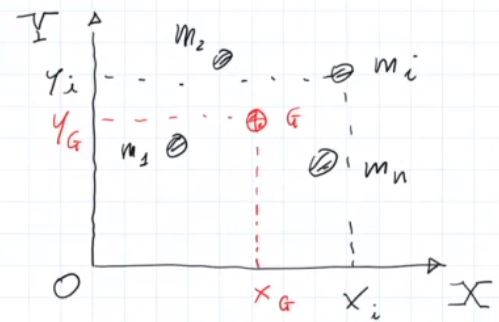
\includegraphics[height=3cm]{../lezione11/img1.JPG}
\end{center}
\[
    \begin{cases}
        \vec{T}_1 = - \vec{T}_2\\
        \vec{N}_1 = - \vec{N}_2
    \end{cases} \rightarrow \begin{cases}
        |\vec{T}_1| = |\vec{T}_2| = T\\
        |\vec{N}_1| = |\vec{N}_2| = N
    \end{cases}
\]
Possiamo ora definire la forza di attrito per il primo corpo come:
\[
    \vec{T}_1 = - f_d N  \frac{\vec{v}_{12}}{|\vec{v}_{12}|} = - f_d N  \frac{\vec{v}_1 - \vec{v}_2}{|\vec{v}_1 - \vec{v}_2|} 
\]
con $f_d$ \textbf{coefficiente di attrito dinamico}, e modulo $ |\vec{T}_1| = f_d N$, mentre direzione $ - \frac{\vec{v}_{12}}{|\vec{v}_{12}|}$ opposta alla velocità di strisciamente del corpo $1$ rispetto al copro $2$, che può essere espresso anche come $\frac{\vec{v}_1 - \vec{v}_2}{|\vec{v}_1 - \vec{v}_2|}$.\newline
[immaigne dagli appunti del prof]
\begin{center}
    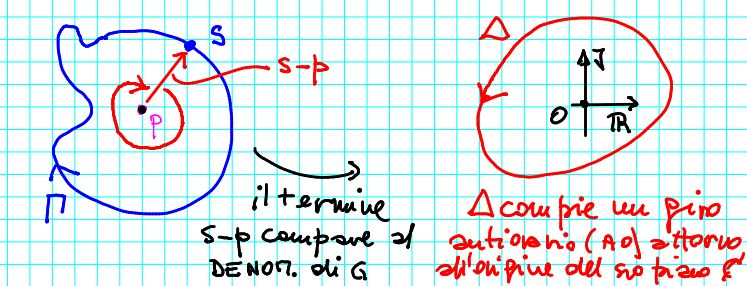
\includegraphics[height=3cm]{../lezione11/img2.JPG}
\end{center}
Notiamo inoltre che $\vec{v}_{12} = - \vec{v}_{21}$ e quindi la formula può essere riscritta come $\vec{T}_1 = f_d N  \frac{\vec{v}_{21}}{|\vec{v}_{21}|}$ .\newline
Porre molta attenzione a questo concetto di velocità relativa, la forza di attrito non dipende dalla velocità di uno solo dei due corpi, ma dalla velocità relativa di entrambi.
\ \newline
Operativamente il termine $N$ viene ricavato imponendo delle equazioni di equilibrio. Il termine $f_d$, che consideremo costante, dipende unicamente dai materiali a contatto, dalla finitura e dall'eventuale presenza di lubrificante. In realtà per velocità relative molto basse, il coefficiente di attrito dinamico non è costante e solitamente $f_d \leq f_s$.\newline
\newline
\subsubsection{Casi particolari}
Ipotiziamo che la velocità del corpo $2$ sia nulla: $\vec{v}_2 = 0$.\newline
[immaigne dagli appunti del prof]
\begin{center}
    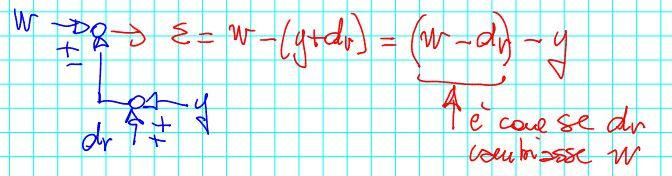
\includegraphics[height=3cm]{../lezione11/img3.JPG}
\end{center}
La forza di attrito sul corpo $1$ vale $|\vec{T}_1| = f_d N$ e la direzione sarà opposta alla velocità, cioè direzione $- \frac{\vec{v}_1}{|\vec{v}_1|}$. Sul secondo corpo quindi apparirà una forza uguale e contraria.\newline
[immagine dagli appunti del prof]
\begin{center}
    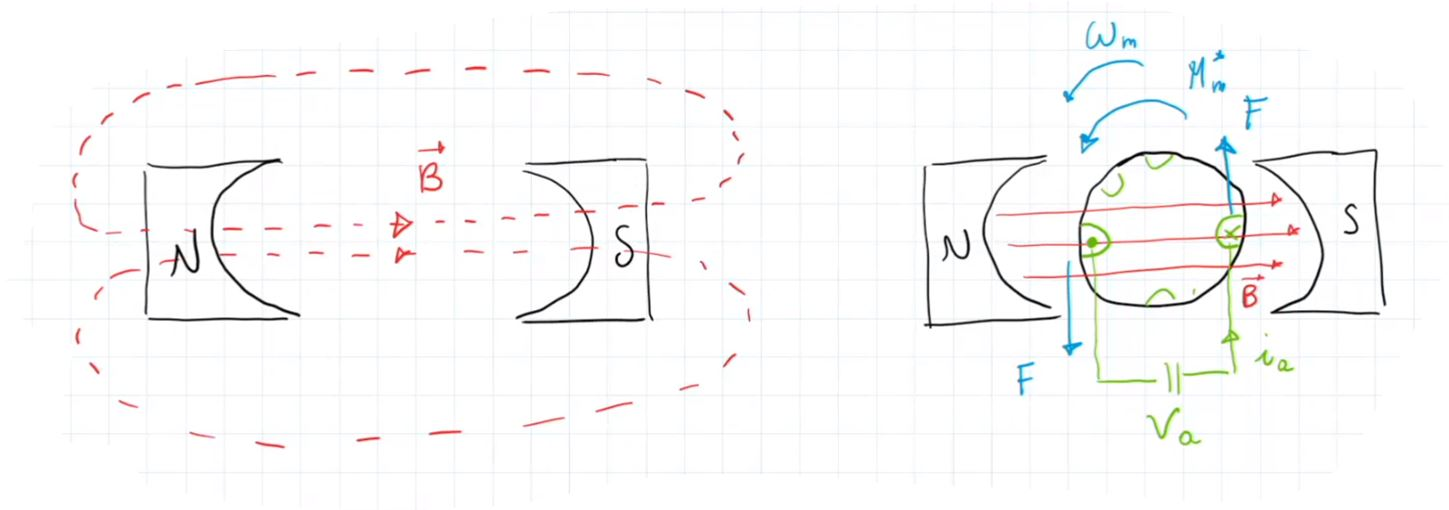
\includegraphics[height=3cm]{../lezione11/img4.JPG}
\end{center}
\ \newline
Ipotiziamo ora il caso contrario, cioè quello in cui $\vec{v}_1 = 0$:\newline
[immagine dagli appunti del prof]
\begin{center}
    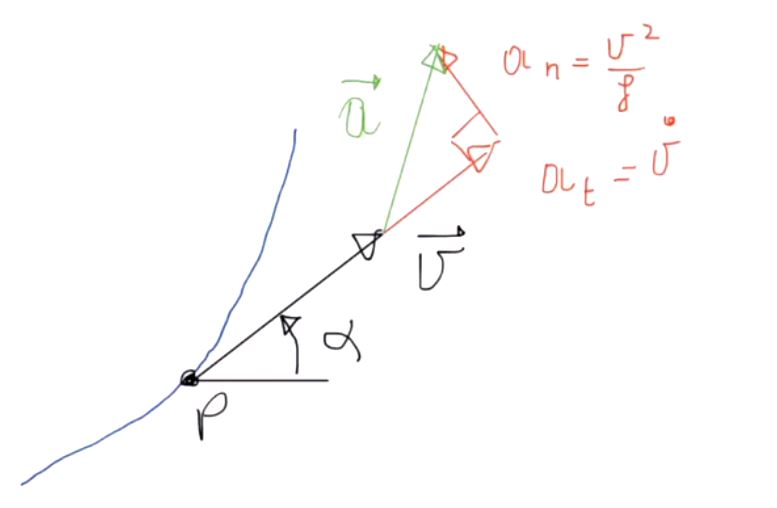
\includegraphics[height=3cm]{../lezione11/img5.JPG}
\end{center}
In questo caso, abbiamo sempre $|\vec{T}_1| = f_d N$, ma la direzione sarà contraria alla direzione di $\vec{v}_{12} = \vec{v}_1 - \vec{v}_2 = - \vec{v}_2$, per cui $\vec{T}_1 = - f_d N \frac{\vec{v}_2}{|\vec{v}_2|}$, quindi in questo caso $T_1$ avrà direzione concorde con $v_2$:\newline
[immagine dagli appunti del prof]
\begin{center}
    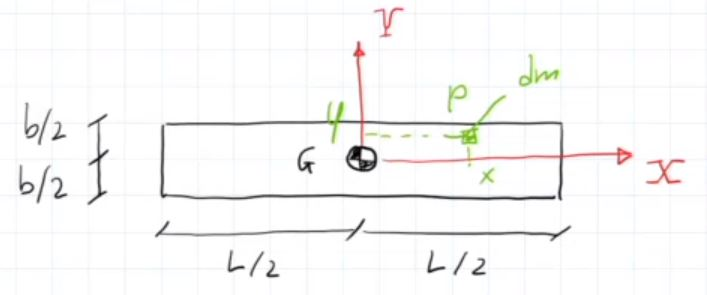
\includegraphics[height=3cm]{../lezione11/img6.JPG}
\end{center}
\ \newline
Vediamo ora un caso più generale, in cui $v_1 > v_2$:\newline
[immagine dagli appunti del prof]
\begin{center}
    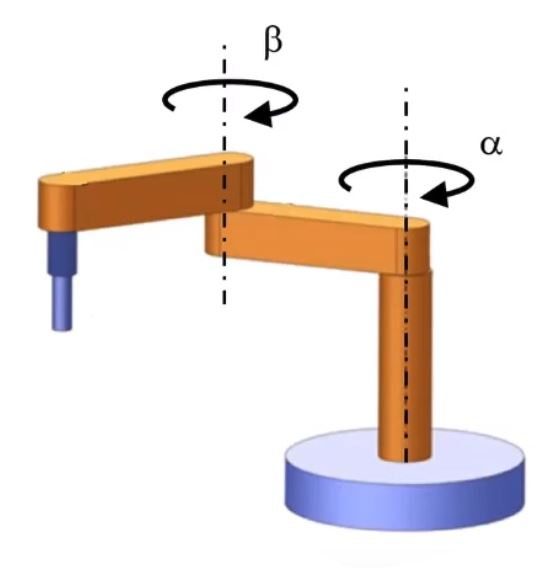
\includegraphics[height=3cm]{../lezione11/img7.JPG}
\end{center}
\ \newline
Nel caso in cui si abbia $\vec{v}_1 = \vec{v}_2$, allora non si ha moto relativo fra i due corpi, quindi si ha attrito statico.
\subsection{Potenza legata alle forze d'attrito}
La potenza legata alle forze d'attrito è sempre una \textbf{potenza dissipata}.\newline
\newline
Vediamo come calcolarla:
\[
    W_d = \vec{T}_1 \;\text{x}\;\vec{v}_1 + \vec{T}_2 \;\text{x}\; \vec{v}_2 + \cancel{\vec{N}_1 \;\text{x}\;\vec{v}_1} + \cancel{\vec{N}_2 \;\text{x}\; \vec{v}_2} 
\]
In cui i termini cancellati sono prodotti vettoriali fra vettori perpendicolari.\newline
Inoltre sapendoche $\vec{T}_2 = - \vec{T}_1$ possiamo scrivere:
\[
    W_d = \vec{T}_1 \; \text{x}\; (\vec{v}_1 - \vec{v}_2) = \vec{T}_1 \;\text{x}\; \vec{v}_{12} = - f_d N \frac{\vec{v}_{12}}{|\vec{v}_{12}|} \;\text{x}\;\vec{v}_{12}
\]
\[
    W_d = - f_d N \frac{v_{12}^2}{|\vec{v}_{12}|} = f_d N |v_{12}|
\]
Siccome $f_d N > 0$ e $|v_{12}| > 0$, allora $- f_d N |v_{12}| <0$, da cui ricaviamo che si tratta di potenza dissipata.
\subsection{Attrito per un disco che rotola su una guida piana}
[immagine dagli appunti del prof]
\begin{center}
    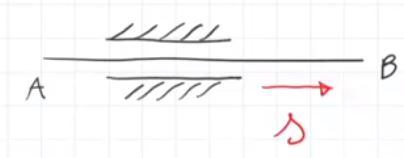
\includegraphics[height=3cm]{../lezione11/img8.JPG}
\end{center}
Considerando i corpi rigidi, il contatto fra disco e piano è di tipo puntiforme e avviene nel punto $C$. Isoliamo i due corpi e notiamo e mostriamo le forze di azione e reazione:\newline
[immagine dagli appunti del prof]
\begin{center}
    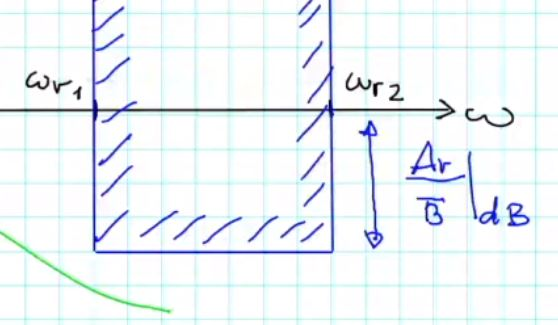
\includegraphics[height=3cm]{../lezione11/img9.JPG}
\end{center}
A questo punto dobbiamo distinguere due casi separati:
\begin{itemize}
    \item \textbf{Puro rotolamento}: Nel caso di puro rotolamento il punto $C$ rappresenta il centro di istantaneo rotolamento, per cui $\vec{v}_C = 0$ e quindi non vi è moto relativo, dunque siamo in condizioni di attrito statico. In questo caso il sistema ha $1$ grado di libertà, il rotolamento.
    \item \textbf{Strisciamento}: In questo caso siamo in presenza di un moto relativo fra i due corpi, e di conseguenza di attrito dinamico. In questo sistema si hanno $2$ gradi di libertà, rotolamento e strisciamento.
\end{itemize}
\ \newline
In pratica, quando stiamo studiando un disco che rotola, dobbiamo ipotizzare le condizioni di puro rotolamento, calcolare le forze $T$ e $N$, imponendo delle equazioni di equilibrio dinamico e infine si verifica la condizione di aderenza, cioè $T \leq T_{lim} = f_s N$. Se questa disuguaglianza è verificata, allora l'ipotesi fatta è corretta, altrimenti le ipotesi sono scorrette, quindi abbiamo moto relativo fra i due corpi (strisciamneto) e saremo in condizioni di attrito dinamico, e quindi i valori di $T$ e $N$ calcolati non vanno bene ($|\vec{T}| = f_d |\vec{N}|$).\newline
\newline
Se siamo in condizione di strisciamento, avremo della potenza dissipata.\newline
Se siamo in condizioni di puro rotolamento, le forze $T$ e $N$ sono applicate al punto $C$, che ha velocità nulla, quindi la potenza dissipata per attrito si annulla:
\[
    W_d = (\vec{T} + \vec{N}) \;\text{x}\; \vec{v}_C = 0
\]
Sperimentalmente però questo risultato non torna, il problema sta nel modello di Coulomb che stiamo utilizzando. Per far fronte a questo problema si utilizza il modello di resistenza al rotolamento.
\subsubsection*{Modello di resistenza al rotolamento}
L'ipotesi alla base di questo modello è che si deve essere in condizioni di puro rotolamento e quindi di attrito statico. Il modello prevede di usare come punto di applicazione della forza $N$, non il punto $C$ di istantanea rotazione, ma un punto $C'$ in avanti di una quantità $u$ rispetto alla direzione del moto del disco.\newline
[immagine dagli appunti del prof]
\begin{center}
    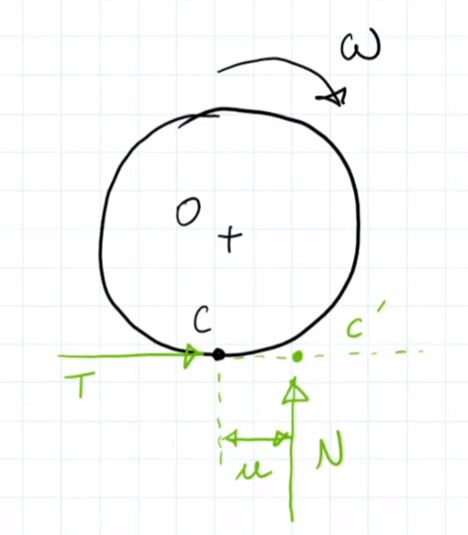
\includegraphics[height=3cm]{../lezione11/img10.JPG}
\end{center}
Interpretando così il punto di applicazione della forza $N$, posso ora spostare nuovamente nel punto $C$ questa forza, aggiungendo ora una componente di momento detto \textbf{momento di trasporto} $C_r$, pari a $N$ moltiplicata per il braccio $u$, questa coppia si oppone alla rotazione del disco e quindi dissipa energia:
\[
    W_d = \vec{C}_r \;\text{x}\; \vec{\omega} = -C_r \omega = - N u \omega < 0
\]
[immagine dagli appunti del prof]
\begin{center}
    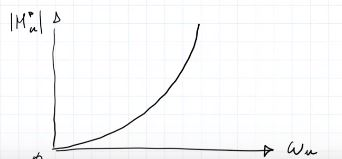
\includegraphics[height=3cm]{../lezione11/img11.JPG }
\end{center}
Generalmente la quantità $u$, cioè la distanza fra $C$ e $C'$, viene espressa in dipendenza del \textbf{coefficiente di attrito evolvente} e del raggio $R$ del disco:
\[
    u = f_v R
\]
Possiamo quindi riscrivere la potenza dissipata come
\[
    W_d = - N u \omega = - N f_v R \omega = - N f_v R \frac{v}{R} = - N f_v v
\]
dove abbiamo considerato che $v = \omega R$ nel moto rotatorio.
\subsection{Bilancio di Potenze (BdP) con attriti}
Quando abbiamo parlato di bilancio di potenze abbiamo fatto come ipotesi che i vincoli fossero perfetti, cioè lisci e senza attrito.\newline
\newline
Per estendere il bilancio di potenze e il teorema dell'energia cinetica a vincoli non perfetti ci basta aggiungere al bilancio di potenza la potenza dissipata dalle forze d'attrito:
\[
    W = W_d + W_{in} = 0
\]
dove sicuramente $W_d$ sarà negativa.\newline
Il teorema dell'energia cinetica sarà invece:
\[
    W + W_d = \frac{dE_c}{dt}
\]
Queste equazioni sono quindi valide per \textbf{vincoli fissi e bilateri} (non perfetti).

    \newline
\newline
\title{LEZIONE 12 20/03/2020}\newline
\textbf{link} \href{https://web.microsoftstream.com/video/05bd4cd5-c99f-4a6c-9334-733e9a60083a?list=user&userId=faa91214-a6f5-40d7-8875-253fd49b8ce1}{clicca qui}\newline
\newline
%\end{comment}
    \title{LEZIONE 12 30/03/2020}\newline
\textbf{link} \href{https://web.microsoftstream.com/video/22a546ac-3e6b-43e0-b0f9-45a630661700?list=user&userId=faa91214-a6f5-40d7-8875-253fd49b8ce1}{clicca qui}
\begin{itemize}
    \item $G_b(s)= \frac{1}{s^g} \rightarrow G(j \omega) = \frac{1}{(j \omega)^g} \rightarrow \begin{cases}
        |G_b(j \omega)| = \frac{1}{\omega^g} \rightarrow |G_b(j \omega)|_{dB}= - 20 g log(\omega)\\
        arg(G_b(j \omega)) = - g \cdot 90^o
    \end{cases} $\newline
    [immagine dagli appunti del prof]\newline \newline
    diagramma di bode del modulo: Il diagramma di bode del modulo corrispondente interseca sempre l'asse delle ascisse nel punto $\omega = 1$ e la pendenza è $-20g \frac{dB}{decade}$ (spesso abbreviato come "pendenza $-g$"), dove la \textbf{decade} è la distanza corrispondente a un rapporto che vale $10$.\newline \newline
    diagramma di bode delle fasi: Il diagramma di bode delle fasi è orizzontale al valore $-g \cdot 90^o$.\newline \newline
    Da notare è che fino ad ora non abbiamo fatto nessuna approssimazione.
    \item $G_c(s)= 1 + st \rightarrow  G_c(j \omega) = 1 + j \omega t \rightarrow \begin{cases}
        |G_c(j \omega)| = \sqrt{1 + (\omega t)^2}\\
        arg(G_c(j \omega))= arctan(\omega t)
    \end{cases}$\newline
    Per facilitare i conti applichiamo un approssimazione, che è il motivo del perchè stiamo facendo diagrammi di bode asintotici:
    \begin{itemize}
        \item se $| \omega t| >> 1$ (molto maggiore di $1$), allora $G_c(j \omega) \sim  j \omega t$, per cui otteniamo \newline che $\begin{cases}
            |G_c(j \omega)| \sim  | \omega t| \\
            arg(G_c(j \omega)) \sim  \begin{cases}
                90^o  \;\;& t>0\\
                -90^o & t <0
            \end{cases}
        \end{cases}$
        \item se $| \omega t| << 1$ (molto minore di $1$), allora $G_c(j \omega) \sim 1$, per cui otteniamo \newline ce $\begin{cases}
            |G_c(j \omega)| \sim  1 \\
            arg(G_c(j \omega)) \sim 0^o
        \end{cases}$
    \end{itemize}
    [immagine dagli appunti del prof]\newline \newline
    diagramma di bode del modulo: Definiamo la \textbf{frequenza d'angolo} $\frac{1}{t}$ nel diagramma di Bode del modulo. Grazie alle approssimazioni che abbiamo fatto, andando a sinistra nell'asse delle $\omega$, cioè verso il valore di $0 _{dB}$, il modulo vale circa $1$. Facciamo valere questa approssiamazione fino al valore di frequenza d'angolo. Superata la frequenza d'angolo il modulo cresce con pendenza $+1$, cioè di $20 \frac{dB}{decade}$. Questa rappresentazione prende il nome di diagramma di bode del modulo asintotico (il diagramma di bode del modulo esatto è mostrato in figura, e la differenza è che non ha una curva "netta").\newline \newline
    diagramma di bode delle fasi:
\end{itemize}
    %esercitazioni
    \newpage
    \part{Esercitazioni}
%\begin{comment}
    \title{LEZIONE 8 02/04/20}\newline
\textbf{link} \href{https://web.microsoftstream.com/video/75f95083-fbf8-4126-8c4d-c65d89f7c6b3}{clicca qui}
\section{Esercitazione}
\subsection{Esercizio bacheca messaggi}
[Su beep troviamo le slide .pptx e i video che commentano la soluzione di questo esercizio e pure il progetto eclipse. In questi appunti non prenderò note in dettaglio sulla soluzione dell'esercizio in quanto su Beep è possibile reperire tutto il materiale necessario. Mi concentrerò di più sugli aspetti chiave e sui concetti fondamentali da usare per risolvere un generico esercizio].\newline
\newline
Per tutti gli esercizi si parte dalla lettura di un testo che rappresenta i requisiti.\newline
\newline
La prima operazione da fare è domandarsi quali sono i dati necessari per il supporto delle funzioni applicative. Per modellare i dati usiamo i concetti che dovrebbero già essere stati appresi durante il corso di basi di dati.\newline
Per l'analisi dei dati si legge il testo e si cercano quelli che possono essere oggetti (entity), attributi degli oggetti (attributes) e proprietà che legano più di un oggetto (relationship).\newline
L'analisi dei dati è un punto critico che spesso gli studenti tralasciano o fanno male e che può portare a sanzioni pesanti. E' bene esercitarsi su questa tecnica.\newline
\newline
Dall'analisi dei dati segue la stesura dello schema concettuale, ovvero il Database design con lo schema entità relazione (da ripassare). Riguardo allo schema entità relazione ricordiamo: le entità sono dei quadrati, hanno degli attributi scritti a fianco e sono legate fra di loro con delle relationship, che sono dei rombi. E' importante segnare sempre le cardinalità (minima:massima)! Usiamo sempre la notazione di Peter Chan (?).\newline
\newline
Ora si usano le regole di Stefano Ceri per la traduzione di uno schema concettuale in uno schema logico in linguaggio ddl (data definition language) SQL. Dobbiamo sempre mostrare le primary keys e le foreign keys. Per le chiavi si cerca sempre di usare un ID numerico con autoincremento (auto fornito dalla base di dati per default), ormai questo è lo standard dei database moderni, non cerchiamo di usare titoli o stringhe articolate come chiavi.\newline
Un errore che spesso accade in esame è che gli studenti si scordano di mostrare lo schema logico (quello in codice).\newline
\newline
Application requirements analysis: l'obbiettivo dell'analisi funzionale delle specifiche per un applicazione web è il cercare i componenti che poi andranno a costituire la nostra applicazione.\newline
Grazie allo schema strutturale diviso in web tier e business and data tier, sappiamo già quali sono i componenti che dobbiamo andare a ricercare.\newline
Utiliziamo un percorso graduale per cercare questi componenti.\newline
Cominciamo a vedere quali sono le interfacce utente (le pagine che abbiamo) e gli eventi che l'utente può scatenare e le azioni che ne corrispondono.\newline
Si cercano le pagine, poi i vari componenti di ciascuna pagina (form, tabelle, etc).\newline
Come terza cosa si cercano gli eventi. L'evento più tipico sono le azioni che si possono fare per interagire con le pagine, esistono anche altri tipi di eventi, come le notifiche, ma solitamente in questi esercizi non ce ne sono. C'è sempre un evento nascosto implicito (non espresso nella specifica) in tutti gli esercizi che è l'accedere all'applicazione.\newline
Come quarta cosa si cercano le azioni, cioè le risposte che l'applicazione ha allo scaturirsi di un evento. Per brevità ignoriamo le azioni di estrazioni di dati dal DB e che sono implicitamente previste dai contenuti dinamici. Focaliziamoci sulle azioni più esplicite come il compilare un form.\newline
\newline
Una volta eseguita l'application requirement analysis, si fa uno schema, un disegno che lo rappresenti. Questo disegno possiamo farlo come ci pare, se ci piace usiamo IFML. L'importante è che si vedano le seguenti cose:
\begin{itemize}
    \item le viste (in IFML sono dei rettangoli);
    \item i componenti delle viste (in IFML sono rettangoli smussati all'interno delle viste);
    \item gli eventi (in IFML sono dei pallini bianchi e con una freccia che mostra cosa succede);
    \item azioni (in IFML sono sono dei rettangoli allungati in cui il lato corto è tipo curvo... non so come spiegarlo, vedi le slide)
\end{itemize}
IFML non è obbligatorio, si può usare qualunque cosa, se volete potete usare IFMLEdit.org per creare dei grafici IFML.\newline
\newline
Fino ad ora abbiamo analizzato il cosa tratterà la nostra applicazione, ora ci occuperemo del come avverrà.\newline
\newline
Per tradurre il nostro schema IFML in qualcosa che mi esprima il come le varie cose verranno fatte, passiamo per l'architettura web-tier e Business and data tier. Il processo è molto facile e dobbiamo solo occuparci di definire gli oggetti di modello (beans), i DAO (data access object, avremo tipicamente un DAO per ogni entità, in più dovremmo analizzare i metodi che ogni DAO deve avere), i controllori (servlet, sono gli eventi) e le viste (template, sono le pagine dell'applicazione).\newline
\newline
Per quanto riguarda il codice effettivo da scrivere su carta all'esame, il professore richiede solo tre cose: per primo tutti i metodi dei DAO, cioè il professore vuole vedere tutto ciò che è legato all'SQL nella nostra applicazione, in più viene solitamente richiesta la stesura di un controllore e di una vista.\newline
\newline
Gli eventi vengono spesso facilmente analizzati con diagrammi di sequenza. Ogni evento a il suo diagramma di sequenza.\newline
E' buona abitudine chiamare eventi che riguardano la restituzione di una vista con il nome "/GoToNomeDellaPagina" (non è un obbligo\dots).\newline
Questi diagrammi non trattano la gestione degli errori. Solitamente si fanno più diagrammi, quelli per scenari regolari e quelli per i casi di errore.
\subsection{Esercizio post management}
Lo scopo di questo secondo esercizio è quello di mostrare un'esercizio in cui la specifica è meno chiara (esposta in maniera meno facile) e la cui implementazione è scritta "meno bene" di quella prima.\newline
\newline
Anche per questo esercizio è possibile reperire tutto il materiale necessario su Beep.\newline
\newline

    \title{LEZIONE 9 15/04/20}
\textbf{link} \href{https://web.microsoftstream.com/video/50d86a59-0bba-4abf-80d2-97c0fc1f39e1?list=user&userId=cfe0965d-9a7c-40e2-be6e-f078296a1914}{clicca qui}
\section{esercizio da un tema d'esame (pt.1)}
    \section{Esercitazione 3}
\title{LEZIONE 10 25/03/2020}\newline
\textbf{link} \href{https://web.microsoftstream.com/video/562a82e0-19cc-4f81-9183-eee77c9c45a4?list=user&userId=faa91214-a6f5-40d7-8875-253fd49b8ce1}{clicca qui} \;\;\textbf{[inizio lezione - 0:26:39]}\newline
\newline
Appunti del prof con annotazioni \url{../pdf/FdA-L10-2020.03.25.pdf} \textbf{[da pagina 0 a pagina 5]}\newline
Contenuto:
\begin{itemize}
    \item Routh.
\end{itemize}
    \section{Esercitazione 4}
\title{LEZIONE 14 1/04/2020}\newline
\textbf{link} \href{https://web.microsoftstream.com/video/7cfe3714-fd1e-453f-8394-f7abd4d747ad?list=user&userId=faa91214-a6f5-40d7-8875-253fd49b8ce1}{clicca qui}\newline
\newline
Appunti del prof con annotazioni \url{../pdf/FdA-L14-2020.04.01.pdf}
%\end{comment}
    \title{LEZIONE 15 07/05/20}
\textbf{link} \href{https://web.microsoftstream.com/video/cc735a4e-c7cb-467d-97bd-910450c2d0a3?list=user&userId=cfe0965d-9a7c-40e2-be6e-f078296a1914}{clicca qui}
\newline
\newline
Function statement: function f()\{\dots;\}; definisce una funzione; la funzione si invoca con l'operatore di chiamata (); deve avere un nome; la funzione è soggetta a "hoisting" per cui è disponibile anche prima di dove è stata definita nel programma.\newline
\newline
Function expression: var f = function ()\{\dots;\};; definisce la variabile f che ha come valore una funzione; non necessita di un nome, ma nel caso in cui venga specificato, il nome è utilizzabile solo all'interno del body della stessa; la funzione è invocata tramite il nome della variabile; la funzione è definita solo quando avviene la valutazione dell'espressione, cioè finchè la riga di codice contenente la variabile f non viene eseguita, la funzione non esiste; la funzione può vedere le variabili dello scope in cui è definita (chiusura).\newline
\newline
Per creare variabili non globali in JavaScript bisogna creare uno scope tramite le funzioni. Mostriamo un esempio:
\begin{lstlisting}
var scope = ( function(){
    var variabileNonGlobale = 0;
    return function(){
        //Possiamo usare la variabile non globale qua per via della chiusura.
    }
})();
\end{lstlisting}
\ \newline
Questa è una cosiddetta "iife", cioè immediately invoked function expression.\newline
Una iife è un'espressione che comporta la dichiarazione e l'esecuzione di una funzione e sono utilizzate per delimitare una porzione di codice evitando che le variabili finiscano nello scope globale.\newline
La presenza delle parentesi tonde esterne (grouping operator) rendono la frase un'espressione valida, altrimenti sarebbe un function statement e non un function expression.\newline
Le iife possono essere usate anche per realizzare un meccanismo di protezione delle variabili, cioè si riesce a imitare il comportamento dei getter e setter di attributi privati:
\begin{lstlisting}
var Sequence = (function sequenceIIFE(){
    var current = 0; //variabile privata
    return { //ritorna un oggetto
        getCurrentValue: function(){
            return current; //rimene vivo per chiusura
        },
        getNextValue: function(){
            current = current +1;
            return current; //rimane vivo per chiusura
        }
    };
})();
\end{lstlisting}
In questo caso la variabile current non è accessibile se non attraverso i metodi Sequence.getCurrentValue() e Sequence.getNextValue().\newline
\newline
Le funzioni possono essere assegnate a proprietà di oggetti (metodi di un oggetto), il parametro this denota l'oggetto su cui la funzione è chiamata, ma un metodo non può usare una funzione innestata che operi direttamente sull'oggetto this, cioè la funzione innestata non condivide il riferimento a this. per permetterle di accedere a this bisogna salvarne un riferimento in una variabile (var self = this;) che sarà visibile nella funzione innestata.\newline
\newline
Invocazione indiretta di funzione: i metodi call e apply di un oggetto di tipo funzione permettono di invocare la funzione, passandogli un valore da usare come this e nel caso di call una lista di argomenti, nel caso di apply un vettore di argomenti.\newline
\newline
L'oggetto arguments è disponibile all'interno delle funzioni quando vengono invocate e contiene i valori dei parametri, include anche i valori opzionali ed è utile per la definizione di funzioni con un numero non specificato di parametri. Notare che arguments non è un vero e proprio vettore, ha la proprietà lenght, ma manca di tutti gli altri metodi tipici dei vettore, si dice essere un oggetto "array-like" o "pseudo-array".\newline
\newline
Una funzione restituisce sempre un valore. Casi speciali:
\begin{itemize}
    \item undefined: se il valore di ritorno non è specificato;
    \item this: se la funzione è un costruttore invocato con l'operatore new.
\end{itemize}
\ \newline
Arrow function: le arrow function sono una notazioen abbreviata per la scrittura di espressioni funzionali. Le uniche differenze sono:
\begin{itemize}
    \item non possiede l'oggetto arguments;
    \item si può usare this, che eredità il valore dalla più vicina funzione normale che la racchiude;
    \item non può essere usata come costruttore con la parola new.
\end{itemize}
\begin{lstlisting}
var add = function(x,y){
    return x + y;
};
//equivale a:
var add = (x,y) => {
    return x + y;
};
\end{lstlisting}
\ \newline
Una funzione di callback è un meccanismo usato per gestire eventi asincroni che causano la chiamata di una funzione:
\begin{itemize}
    \item la funzione da chiamare è passata come parametro alla funzione che gestisce l'evento;
    \item la funzione passata come parametro è invocata quando l'evento si manifesta.
\end{itemize}
Un tipico esempio sono le richieste HTTP asincrone al server.
\newline
\newline
    \section{Esercitazione 6}
\title{LEZIONE 16 6/04/2020}\newline
\textbf{link} \href{https://web.microsoftstream.com/video/0384d9d2-5ddc-4381-8933-f46dc8fca4d3?list=user&userId=faa91214-a6f5-40d7-8875-253fd49b8ce1}{clicca qui}\newline
\newline
Appunti del prof con annotazioni \url{../pdf/FdA-L16-2020.04.06.pdf}\newline
Contenuto:
\begin{itemize}
    \item 
\end{itemize}
    \section{Esercitazione 7}
\title{LEZIONE 17 8/04/2020}\newline
\textbf{link} \href{}{clicca qui}\newline
\newline
Appunti del prof con annotazioni \url{../pdf/FdA-L16-2020.04.06.pdf}\newline
Contenuto:
\begin{itemize}
    \item 
\end{itemize}
\end{document}